%%%%%%%%%%%%%%%%%%%%%%%%%%%%%%%%%%%%%%%%%
% "ModernCV" CV and Cover Letter
% LaTeX Template
% Version 1.11 (19/6/14)
%
% This template has been downloaded from:
% http://www.LaTeXTemplates.com
%
% Original author:
% Xavier Danaux (xdanaux@gmail.com)
%
% License:
% CC BY-NC-SA 3.0 (http://creativecommons.org/licenses/by-nc-sa/3.0/)
%
% Important note:
% This template requires the moderncv.cls and .sty files to be in the same 
% directory as this .tex file. These files provide the resume style and themes 
% used for structuring the document.
%
%%%%%%%%%%%%%%%%%%%%%%%%%%%%%%%%%%%%%%%%%

%----------------------------------------------------------------------------------------
%	PACKAGES AND OTHER DOCUMENT CONFIGURATIONS
%----------------------------------------------------------------------------------------
\documentclass[11pt,a4paper,sans]{moderncv} % Font sizes: 10, 11, or 12; paper sizes: a4paper, letterpaper, a5paper, legalpaper, executivepaper or landscape; font families: sans or roman

\moderncvstyle{banking} % CV theme - options include: 'casual' (default), 'classic', 'oldstyle' and 'banking'
\moderncvcolor{blue} % CV color - options include: 'blue' (default), 'orange', 'green', 'red', 'purple', 'grey' and 'black'

\usepackage[utf8]{inputenc}
\usepackage[scale=0.8]{geometry}
%\usepackage[top=0.5cm, bottom=0.5cm, left=1.5cm, right=1.5cm]{geometry} 

%\usepackage[T1]{fontenc}
%\usepackage{parcolumns}
\usepackage{comment}
%\usepackage{url}
\usepackage{eurosym}
\usepackage{multibib}
\newcites{article,conf,confnoproc}{{International journal articles},{International conferences with proceedings}, {International conferences without proceedings}}



\patchcmd{\makehead}
{\hfil}
{\hspace*{0.15\textwidth}}
{}
{}
\patchcmd{\makehead}
{\setlength{\makeheaddetailswidth}{0.8\textwidth}}
{\setlength{\makeheaddetailswidth}{0.67\textwidth}}
{}
{}
\patchcmd{\makehead}
{\\[2.5em]}
{\hfil\raisebox{-.7cm}{\framebox{\includegraphics[width=\@photowidth]{\@photo}}}\\[2.5em]}
{}
{}

\newcommand*{\httpslink}[2][]{% <=======================================
	\ifthenelse{\equal{#1}{}}%
	{\href{https://#2}{#2}}%
	{\href{https://#2}{#1}}}

\newcommand*{\googlescholarsocialsymbol}  {
\includegraphics[width=0.27cm]{logo_scholar}~} % <===================
\newcommand*{\researchgatesocialsymbol}  {
\includegraphics[width=0.27cm]{logo_researchgate}~} % <===================

\makeatletter
\RenewDocumentCommand{\social}{O{}O{}m}{%
	\ifthenelse{\equal{#2}{}}%
	{ 
		\ifthenelse{\equal{#1}{linkedin}}{\collectionadd[linkedin]{socials}{\protect\httpslink[#3]{www.linkedin.com/in/#3}}}{}%
		\ifthenelse{\equal{#1}{googlescholar}}{\collectionadd[googlescholar]{socials}{\protect\httpslink[#3]{www.googlescholar.com/profile/#3}}}{}% <================================================================
		\ifthenelse{\equal{#1}{researchgate}}{\collectionadd[researchgate]{socials}{\protect\httpslink[#3]{www.researchgate.com/profile/#3}}}{}% <================================================================
		\ifthenelse{\equal{#1}{twitter}} {\collectionadd[twitter]{socials} {\protect\httpslink[#3]{www.twitter.com/#3}}}    {}%
		\ifthenelse{\equal{#1}{github}}  {\collectionadd[github]{socials}  {\protect\httpslink[#3]{www.github.com/#3}}}     {}%
	}
	{\collectionadd[#1]{socials}{\protect\httpslink[#3]{#2}}}}
\makeatother

\newcommand{\cvdoublecolumn}[2]{%
	\cvitem[0.75em]{}{%
		\begin{minipage}[t]{\listdoubleitemcolumnwidth}#1\end{minipage}%
		\hfill%
		\begin{minipage}[t]{\listdoubleitemcolumnwidth}#2\end{minipage}%
	}%
}

% usage: \cvreference{name}{address line 1}{address line 2}{address line 3}{address line 4}{e-mail address}{phone number}
% Everything but the name is optional
% If \addresssymbol, \emailsymbol or \phonesymbol are specified, they will be used.
% (Per default, \addresssymbol isn't specified, the other two are specified.)
% If you don't like the symbols, remove them from the following code, including the tilde ~ (space).

\newcommand{\cvreference}[7]{%
	\textbf{#1}\newline% Name
	\ifthenelse{\equal{#2}{}}{}{\addresssymbol~#2\newline}%
	\ifthenelse{\equal{#3}{}}{}{#3\newline}%
	\ifthenelse{\equal{#4}{}}{}{#4\newline}%
	\ifthenelse{\equal{#5}{}}{}{#5\newline}%
	\ifthenelse{\equal{#6}{}}{}{\emailsymbol~\texttt{#6}\newline}%
	\ifthenelse{\equal{#7}{}}{}{\phonesymbol~#7}}

\makeatletter\renewcommand*{\bibliographyitemlabel}{\@biblabel{\arabic{enumiv}}}\makeatother

%\setlength{\hintscolumnwidth}{3cm} % Uncomment to change the width of the dates column
%\setlength{\makecvtitlenamewidth}{10cm} % For the 'classic' style, uncomment to adjust the width of the space allocated to your name

%----------------------------------------------------------------------------------------
%	NAME AND CONTACT INFORMATION SECTION
%----------------------------------------------------------------------------------------

\name{Andrea}{Brugnoli}
%\address{103 rue Bonnat}{Toulouse}{France}% optional, remove / comment the line if not wanted; the "postcode city" and "country" arguments can be omitted or provided empty
\phone[mobile]{+33~7~50~39~47~27}                   % optional, remove / comment the line if not wanted; the optional "type" of the phone can be "mobile" (default), "fixed" or "fax"
\email{andrea.brugnoli92@gmail.com}                               % optional, remove / comment the line if not wanted
%\homepage{www.johndoe.com}                         % optional, remove / comment the line if not wanted
%\social[linkedin]{john.doe}                        % optional, remove / comment the line if not wanted
%\social[twitter]{jdoe}                             % optional, remove / comment the line if not wanted
%\social[github]{andreabrugnoli}                              % optional, remove / comment the line if not wanted
\social[googlescholar][scholar.google.com/citations?user=aze4Eh4AAAAJ&hl=it]{andrea.brugnoli} % <====================================
\social[researchgate][www.researchgate.net/profile/Andrea_Brugnoli2]{andrea.brugnoli}
%\extrainfo{additional information}                 % optional, remove / comment the line if not wanted
\photo[75pt][0.4pt]{Foto_Cv_cropped}   


%\AtBeginDocument{\hypersetup{baseurl={}}}

%----------------------------------------------------------------------------------------

\begin{document}

\makecvtitle % Print the CV title
\begin{comment}
\begin{minipage}{.8\linewidth}
{\huge{\textsc{Andrea BRUGNOLI}}}

\vspace{2mm}
{103 rue Bonnat, 31400 Toulouse (FR)}

{(+33) 7 50 39 47 27}

{ Andrea.BRUGNOLI@supaero.isae.fr or andrea.brugnoli92@gmail.com}

\vspace{1pt}
\homepage{staff.org.edu/~jsmith}{staff.org.edu/$\sim$jsmith} % The first argument is the url for the clickable link, the second argument is the url displayed in the template - this allows special characters to be displayed such as the tilde in this example


\fcolorbox{cyan}{white}{%
\parbox{\textwidth}{\textbf{Phd candidate at ISAE-Supaero (Toulouse)} \newline
\vspace{1mm}
International spirit, initiative and ability to adapt. Fluent in three languages.
}}
\end{minipage}
\begin{minipage}{.2\linewidth}
\begin{center}
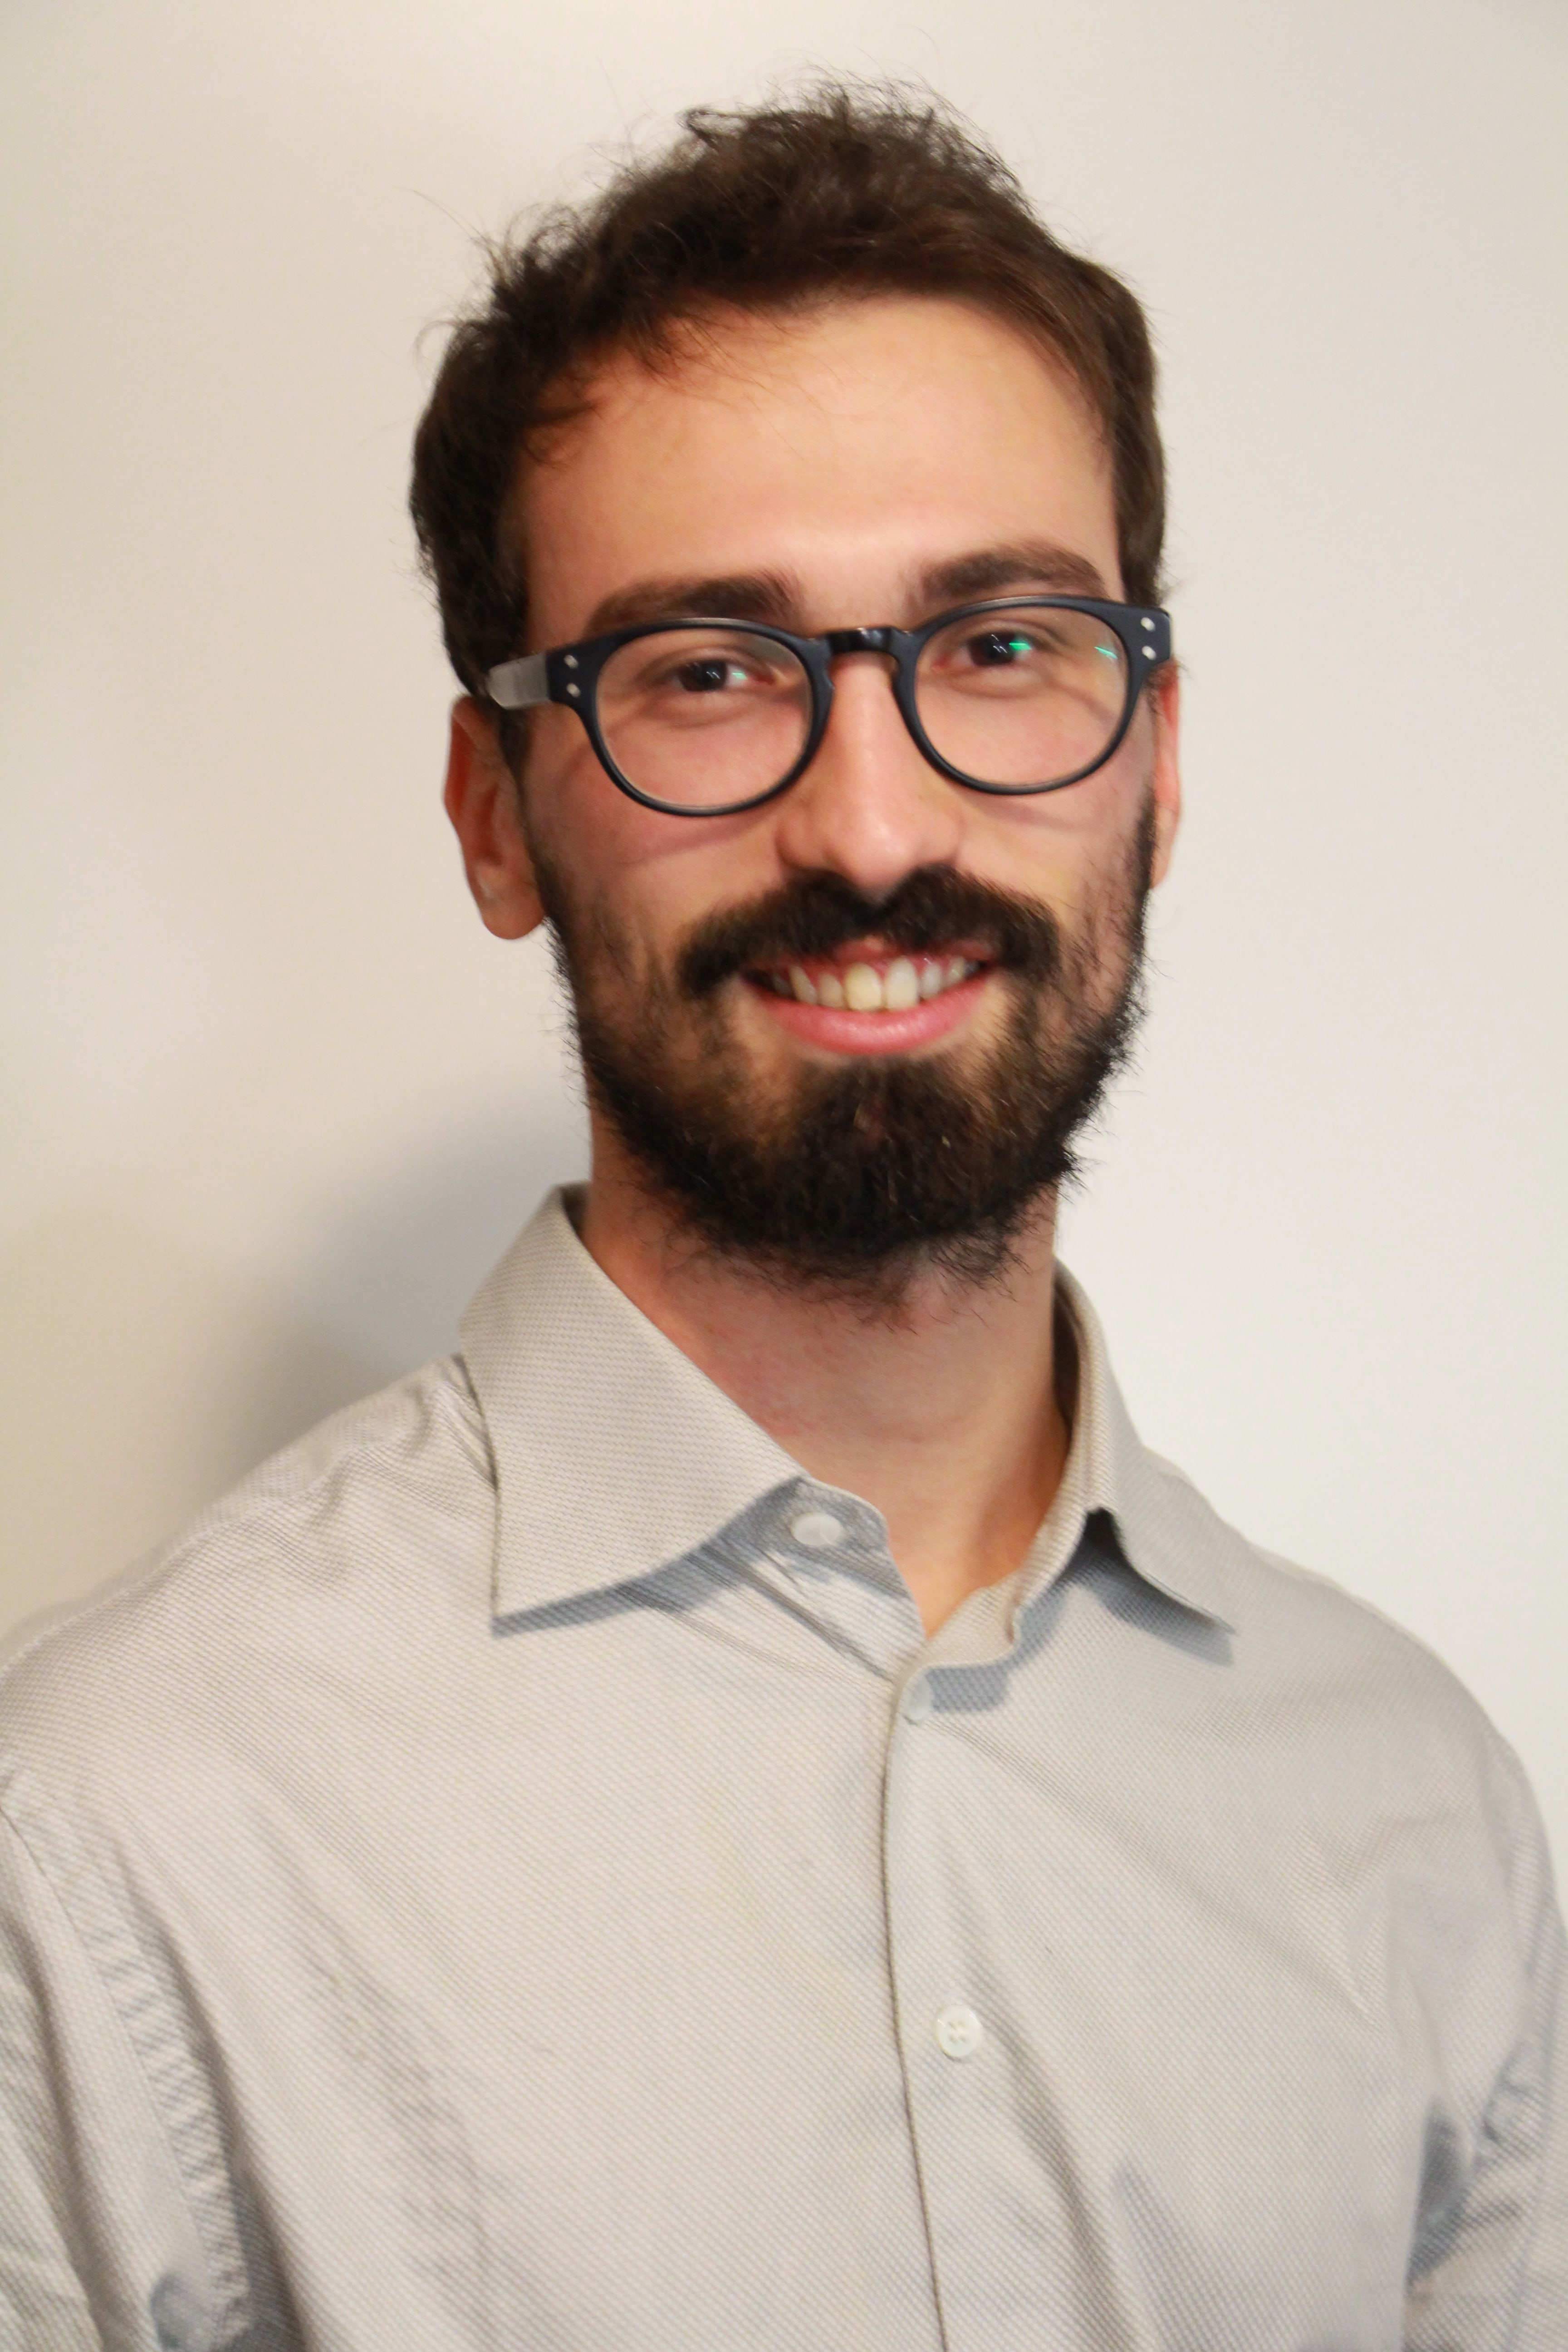
\includegraphics[width=0.8\linewidth]{Foto_Cv-min.jpg}
\end{center}
\end{minipage}
\vspace{3mm}
\end{comment}

%----------------------------------------------------------------------------------------
%	EDUCATION SECTION
%----------------------------------------------------------------------------------------
\section{Academic Positions}
\cventry{November 2020-November 2022}{Post-Doctoral researcher}{University of Twente}{Enschede}{}{Numerical methods for coupled port-Hamiltonian fluid-structure dynamics\\
	ERC Advanced grant. Principal investigator: Stefano Stramigioli}


\section{Education}

% usage: \cventry[spacing]{years}{degree/job title}{institution/employer}{localization}{optionnal: grade/...}{optional: comment/job description}

\cventry{2017-2020}{PhD in Automatic Control}{ISAE-Supaero}{Toulouse}{}{A port-Hamiltonian formulation of flexible structures: modelling and symplectic finite element discretization.\\
Supervisors: Daniel Alazard, Val\'erie Pommier-Budinger and Denis Matignon.}

\cventry{2016--2017}{Research Master in automatics and image processing}{Universit\'{e} Paris Saclay/\,Sup\'{e}lec}{Paris/Toulouse}{}{Courses: inverse problem, advanced dynamics of flexible structures, parameter estimation.}

\cventry{2015--2017}{Double degree in aerospace and astronautical engineering}{ISAE-Supaero}{Toulouse}{}{Specialisation in applied mathematics and advanced automatics: multidisciplinary optimisation, high performance computing, control of flexible structures.}


\cventry{2014--2017}{Master in space engineering}{Politecnico di Milano}{Milan}{\textit{110/110 cum laude} }{
Courses: orbital mechanics, structural dynamics and control, thermochemical propulsion.}


\cventry{2011--2014}{Mechanical Engineering Degree}{Politecnico di Milano}{Milan}{\textit{110/110 cum laude} }{Courses: finite element method, mechanical vibrations, numerical methods for engineering.}

%\cventry{2006--2011}{High school diploma}{Liceo Classico Scipione Maffei}{Verona}{\textit{100/100}}{}

\vspace{1mm}

%----------------------------------------------------------------------------------------
%	WORK EXPERIENCE SECTION
%----------------------------------------------------------------------------------------

\section{Experiences}

\cventry{July 2021}{Summer school in Artificial Intelligence and Reinforcement Learning}{Institut CIFAR}{Toronto, Canada}{}{}

\cventry{January 2019, 4 months}{Visiting researcher}{ITA-Instituto Tecnol\'{o}gico de Aeron\'{a}utica}{S\~{a}o Jos\'{e} dos Campos}{}{Collaboration with Flavio Cardoso-Riberio on numerical methods for port-Hamiltonian systems.}

\cventry{2017, 6 months}{Internship}{CNES-Centre  des études spatiales}{Toulouse}{}{Analysis of dismissed satellites subjected to solar pressure to identify stable and periodic pointing configurations.}

%\cventry{2016, 5 months}{Industrial and entrepreneurial project}{ISAE-Supaero in partnership with LAAS}{Toulouse}{}{Intelligent teleoperations and optimal control for micro-drones systems (six people team).}

%\cventry{2016, 4 months}{Research project}{ISAE-Supaero}{Toulouse}{}{Modular modelling of rigid multibody systems following the logic of Simscape Multibody.}

%\cventry{2015, 2 months}{Interplanetary transfer}{Politecnico di Milano}{Milano}{}{\' 
%Study of optimal trajectories with gravity assist to minimise propellant usage. Perturbation analysis on operational orbit.}

\cventry{2014, 3 months}{Bachelor project}{Politecnico di Milano in  partnership with Danieli S.p.A}{Milan}{} {Dynamics of a forging manipulator. Project selected for the final presentation at Danieli.}

%\cventry{2014, 3 months}{Fem analysis of a mechanical component}{Politecnico di Milano}{Milano}{}{Implementation on Abaqus, equivalent model coded on Matlab , results validation and comparison.}

%\cventry{}{Horizontal Axis Wind Turbine Design}{Politecnico di Milano}{Milano}{}{General sizing, performances optimization nominal point, performance analysis off design. Team of four. Published on Academia  \textcolor{blue}{\texttt{\href{https://www.academia.edu/9561531/Horizontal_Axis_Wind_Turbine_Design}{Horizontal Axis Wind Turbine Design}}} }

%----------------------------------------------------------------------------------------
%	COMPUTER SKILLS SECTION
%----------------------------------------------------------------------------------------

%----------------------------------------------------------------------------------------
%	COMMUNICATION SKILLS SECTION
%----------------------------------------------------------------------------------------

% \section{Communication Skills}

% \cvitem{2010}{Oral Presentation at the California Business Conference}
% \cvitem{2009}{Poster at the Annual Business Conference in Oregon}

%----------------------------------------------------------------------------------------
%	LANGUAGES SECTION
%----------------------------------------------------------------------------------------
\begin{minipage}[t]{0.44\linewidth}
\section{Languages}
\cvitem{English}{fluent}
\cvitem{French}{fluent}
\cvitem{Spanish}{intermediate}
\cvitem{Portuguese}{intermediate}
\cvitem{Italian}{native speaker}
\end{minipage}
\begin{minipage}[t]{0.55\linewidth}
\section{Computer skills}
\cvitem{Softwares and platforms}{Simulink, Abaqus, Inventor, Solid Works, Labview}
\cvitem{Languages}{Python (especially FEM librairies: FEniCS and Firedrake), Matlab, Java, C, \LaTeX}
\cvitem{OS}{Linux environment (Fedora, Ubuntu)}
\end{minipage}


%----------------------------------------------------------------------------------------
% Awards
%----------------------------------------------------------------------------------------

\section{Awards}

\cventry{2021}{PHD Thesis Award}{Fondation ISAE-SUPAERO}{}{}{}
\cventry{2011-2017}{Tuition fee waiver for academic merit.}{Politecnico di Milano}{}{}{}



%----------------------------------------------------------------------------------------
%	PUBLICATIONS AND REFERENCES SECTION
%----------------------------------------------------------------------------------------

%\nocite{companion,bertram,cicero,augustine}
\section{References}

\cvdoublecolumn{
	\cvreference{Denis Matignon}
	{Department of Applied Mathematics}
	{ISAE-Supaero}
	{Toulouse, 31055 (FR)}
	{10 Avenue Edouard Belin}
	{denis.matignon@isae.fr}
	{0033-661741511}\\[1em]
	\cvreference{Daniel Alazard}
	{Department of Space and Aeronautics Vehicle Dynamics}
	{ISAE-Supaero}
	{Toulouse, 31055 (FR)}
	{10 Avenue Edouard Belin}
	{daniel.alazard@isae.fr}
	{0033-634981322}\\[1em]
}
{\cvreference{Paul Kotyzca}
	{Department of Mechanical Engineering}
	{Technical University of Munich}
	{Munich, 85748 (GE)}
	{Boltzmannstr. 15}
	{kotyczka@tum.de}
	{}\\[1em]
	\cvreference{Stefano Stramigioli}
	{Robotics \& Mechatronics}
	{University of Twente}
	{Enschede, 7522 NB (NL)}
	{Drienerlolaan 5}
	{s.stramigioli@utwente.nl}
	{}
}

\section{Publications}
{
	\nocitearticle{brugnoli2019ammmin,brugnoli2019ammkir,brugnoli2020msd,brugnoli2021ther,brugnoli2021num,califano2021,brugnoli2022df}
	\bibliographystylearticle{unsrt}
	\bibliographyarticle{biblio_articles}
	
	\nociteconf{brugnoli2019cpde,brugnoli2019cdc,cardoso2019cdc,brugnoli2020wc,brugnoli2020mtns,brugnoli2021vk,cherifi2021data,rashad2021ext}
	\bibliographystyleconf{unsrt}
	\bibliographyconf{biblio_conf}  
	
	\nociteconfnoproc{brugnoli2021siamcse}
	\bibliographystyleconfnoproc{unsrt}
	\bibliographyconfnoproc{biblio_confnoproc}   
}             % 'cv_bibliography' is the name of a BibTeX file


\end{document}










